% Chapter Template

\chapter{Diseño e Implementación} % Main chapter title

\label{Chapter3} % Change X to a consecutive number; for referencing this chapter elsewhere, use \ref{ChapterX}

A continuación se describe el hardware seleccionado para la ampliación del circuito cargador, los criterios tomados en cuenta, el diseño del circuito y su conexión en \ref{sec:hard}. Luego se describe la arquitectura del sistema en \ref{sec:arq} y entra mas en detalle en \ref{sec:firm}, donde muestra un pseudocódigo del \textit{firmware} para explicar su funcionamiento.

%----------------------------------------------------------------------------------------
%	SECTION 1
%----------------------------------------------------------------------------------------
\section{Hardware}
\label{sec:hard}

%-----------------------------------
%	SUBSECTION 1
%-----------------------------------
\subsection{El panel solar}

El sistema fotovoltaico propuesto originalmente estaba basado en módulos con voltaje de 12V y 0.5A. En el mercado existen distintas soluciones comerciales que se ajustan a las necesidades de cada aplicación.

Como medida de mitigación de riesgos, se planteó emplear componentes disponibles en el mercado local, y luego de tener en cuenta factores como costos, tiempo de entrega, soporte pos-venta y al ser de Industria Argentina, se seleccionó el \textit{módulo fotovoltaico policristalino de alto rendimiento KS10T} \footnote{http://www.solartec.com.ar/documentos/productos/3-25wp/SOLARTEC-KS10T-v13.pdf} de la figura \ref{fig:ks10t} de Solartec \footnote{http://www.solartec.com.ar/}. Se trata de paneles fabricados en base a celdas de silicio policristalino de alta eficiencia. La eficiencia de estas celdas es superior al 14\%. Sus características se muestran en la tabla \ref{tab:ks10t} y figura \ref{fig:mecanicas} \footnote{Fuente: SOLARTEC S.A. Todas las distancias están expresadas en mm.}.

 \begin{figure}[h!]
	\centering
    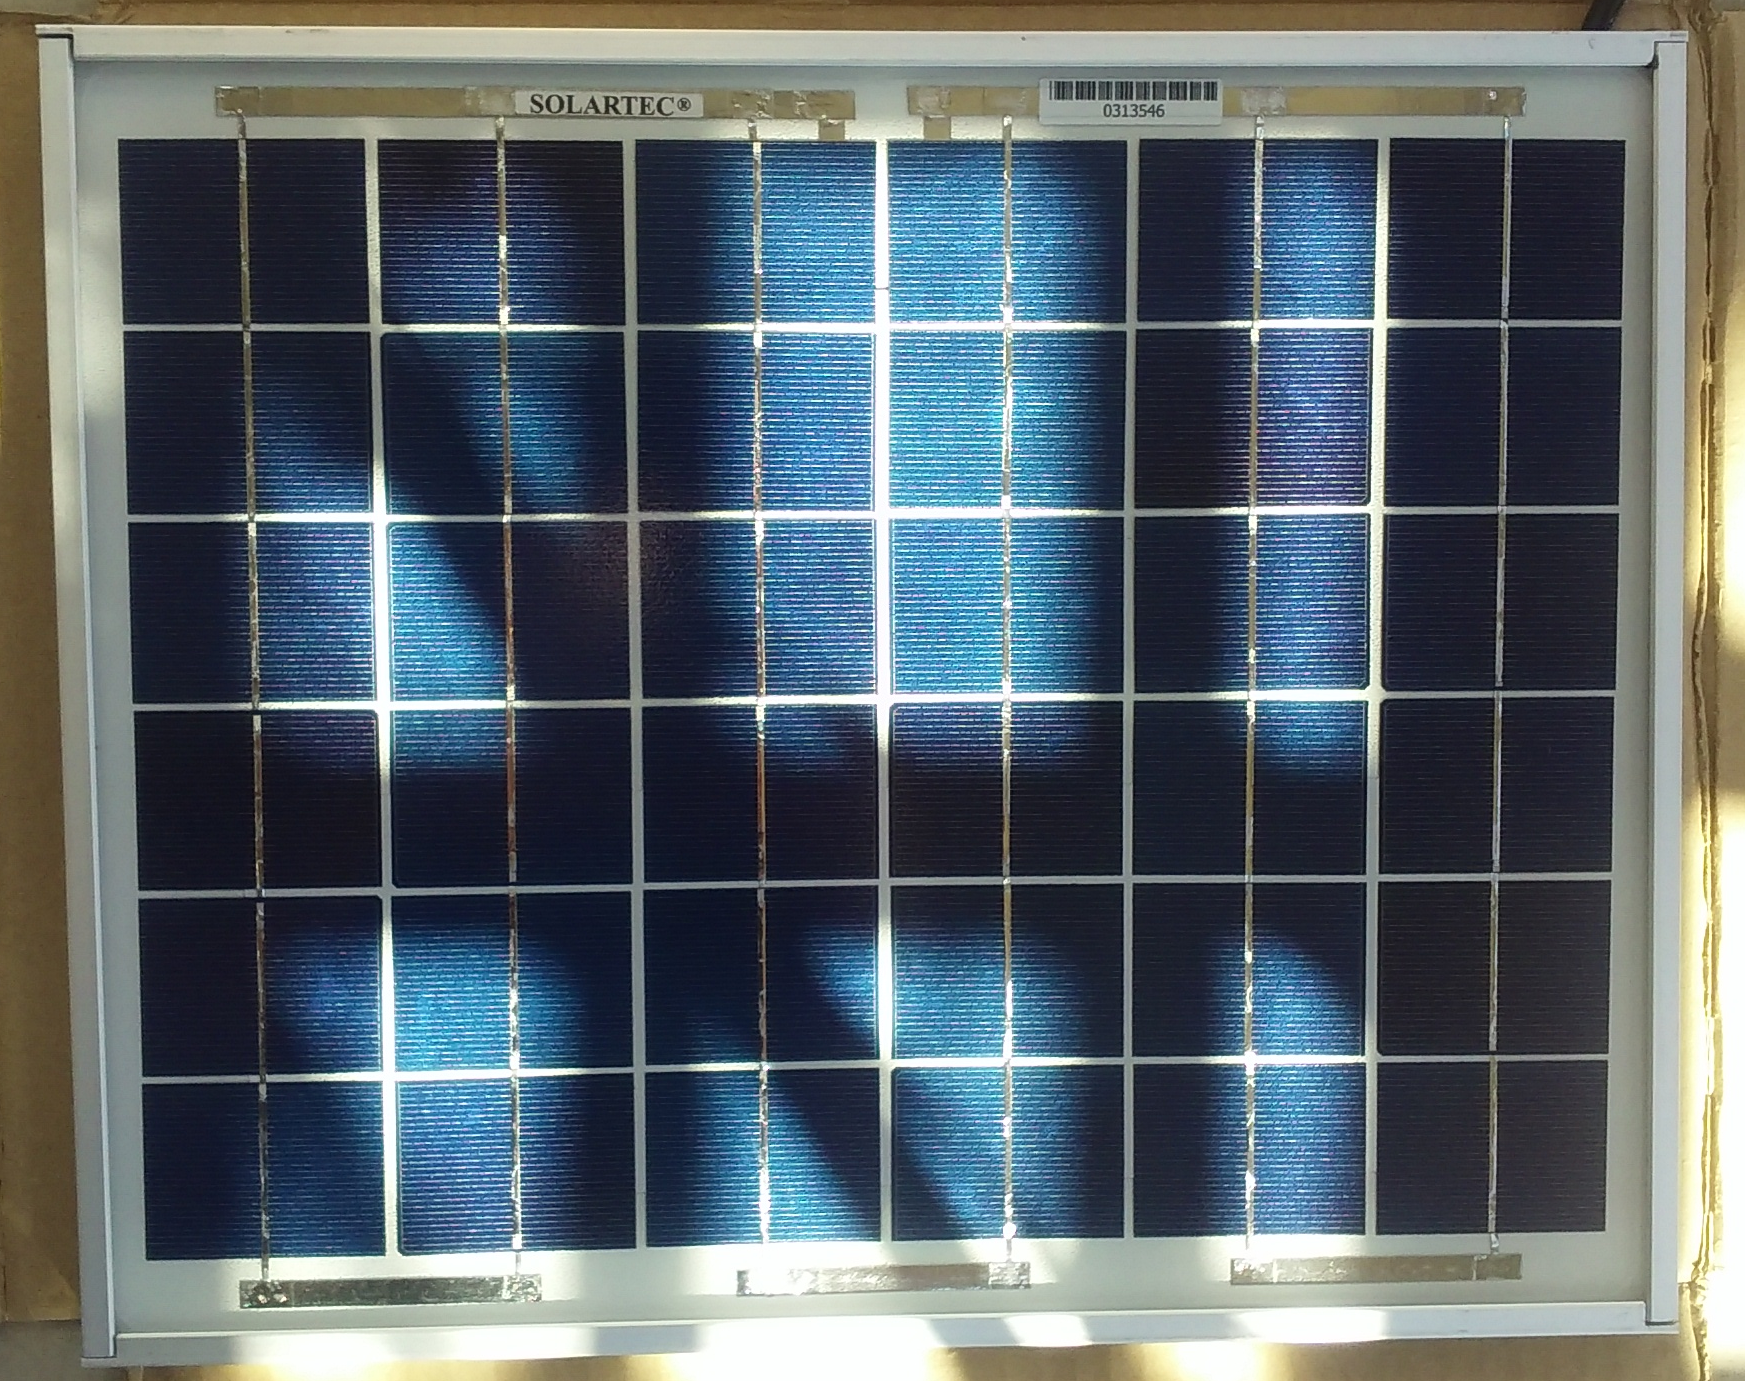
\includegraphics[width=0.5\textwidth]{./Figures/panel.png}
	\label{fig:ks10t}
	\caption{Módulo Fotovoltaico policristalino de alto rendimiento KS10T.}
\end{figure}

\vspace{10px}

\begin{table}[ht]
	\centering
	\caption{Características del módulo fotovoltaico KS10T}
	\begin{tabular}{@{} l *2c @{}}    \toprule
		\emph{\textbf{Características}} & \emph{\textbf{Valor}} & \emph{\textbf{Unidad}}\\
		\midrule
		Potencia nominal	& 10 	& Wp	\\	
		Tensión a PN		& 17.4	& V\\
		Corriente a PN	& 0.58		& A\\
		Dimensiones		& 301x352x22 	& mm\\
		Peso				& 0.58		& Kg	\\
		\bottomrule
		\hline
	\end{tabular}
	\label{tab:ks10t}
\end{table}

\begin{figure}[h!]
	\centering
    \includegraphics[width=0.5\textwidth]{./Figures/mecanicas.JPG}
	\label{fig:mecanicas}
	\caption{Características mecánicas.}
\end{figure}

%\footnote{Fuente: SOLARTEC S.A. Todas las distancias están expresadas en mm.}

La curva de la figura \ref{fig:ks10t}\footnote{Fuente: SOLARTEC S.A.}, muestra la corriente máxima de cortocircuito y la tensión máxima a circuito abierto del \textit{módulo KS10T}. Notese que es capaz de entregar la tensión hasta exigir el máximo de corriente. Los valores y la curva están dados para las condiciones de insolación de 1 KW/m2, masa atmosférica 1.5 y temperatura de celda de 25 \grados C.

\begin{figure}[h!]
	\centering
    \includegraphics[width=0.5\textwidth]{./Figures/curva.JPG}
	\label{fig:curva}
	\caption{Características eléctricas.}
\end{figure}


%-----------------------------------
%	SUBSECTION 2
%-----------------------------------
\subsection{Extensión de circuito cargador}
\label{sec:extensión}
Entre las interfaces para el usuario del nodo \textit{Mote LSE} esta el puerto USB, el cual alimenta al circuito de control de carga \textit{bq24080 1-A} con 5V(DC) a través de un conector USB micro-B. Este circuito es el empleado para la carga de la batería de Li-ion de 3.7V y 900mAh.

Es por esto, que es necesario emplear una etapa reguladora de voltaje a la salida del panel. Para la cual se utiliza el clásico regulador de Fairchild \textit{LM7805} \footnote{https://www.fairchildsemi.com/datasheets/LM/LM7805.pdf} de 1A. Que con unos pocos componentes (un condensador electrolítico como filtro a tierra para señales continuas para moderar la tensión eléctrica y las fluctuaciones de corriente y un condensador de poliéster para filtrar las señales espúreas de alta frecuencia, a la entrada y a la salida), entrega una salida de voltaje entre 4.75V y 5.25V. Además, ofrece protección contra sobrecarga térmica y cortocircuitos y opera entre -40 \grados C y +125 \grados C.

\begin{figure}[h!]
	\centering
    \includegraphics[width=1\textwidth]{./Figures/circuito.jpg}
	\label{fig:circuito}
	\caption{Diseño de extensión de circuito cargador}
\end{figure}

%-----------------------------------
%	SUBSECTION 3
%-----------------------------------
\subsection{Diagrama de conexión}
\label{sec:conexión}

%----------------------------------------------------------------------------------------
%	SECTION 2
%----------------------------------------------------------------------------------------

\section{Arquitectura}
\label{sec:arq}

%-----------------------------------
%	SUBSECTION 1
%-----------------------------------
\subsection{Modelo de Capas}

%-----------------------------------
%	SUBSECTION 2
%-----------------------------------
\subsection{Diagrama en bloques}

Arquitectura modular. Módulos. APIs, interfaces.



%----------------------------------------------------------------------------------------
%	SECTION 3
%----------------------------------------------------------------------------------------
\section{Firmware}
\label{sec:firm}

%-----------------------------------
%	SUBSECTION 1
%-----------------------------------
\subsection{Funcionalidades por capas}

\begin{itemize}
	\item Implementación de funcionalidades en la subcapa MAC

	\item Implementación de funcionalidades en la subcapa PHY

	\item Implementación de funcionalidades a nivel de aplicación
	
\end{itemize}

%-----------------------------------
%	SUBSECTION 2
%-----------------------------------
\subsection{Ajustes a Microstack}


%-----------------------------------
%	SUBSECTION 3
%-----------------------------------
\subsection{Diagramas de topologías implementadas}

\begin{figure}[h!]
	\centering
    \includegraphics[width=.8\textwidth]{./Figures/topologia.jpg}
	\label{fig:topo}
	\caption{1) Topología estrella. 2)Topología Peer-to-Peer}
\end{figure}

\begin{figure}[h!]
	\centering
    \includegraphics[width=.8\textwidth]{./Figures/cluster.jpg}
	\label{fig:clust}
	\caption{Topología árbol de cluster}
\end{figure}

%-----------------------------------
%	SUBSECTION 4
%-----------------------------------
\subsection{Principales funciones}

Funciones

